% !TEX encoding = UTF-8
% !TEX TS-program = pdflatex
% !TEX root = ../tesi.tex
% !TEX spellcheck = it-IT

%**************************************************************
\chapter{Descrizione dello stage}
\label{cap:descrizione-stage}
%**************************************************************

\intro{Breve introduzione al capitolo}\\
Questo capitolo tratterà l'organizzazione temporale del progetto, ovvero la sua divisione in attività e l'estensione temporale di ognuna. Il progetto è stato diviso in quattro fasi distinte, con diverse attività.

%**************************************************************
\section{Introduzione al progetto}

%**************************************************************
%\section{Analisi preventiva dei rischi}

%Durante la fase di analisi iniziale sono stati individuati alcuni possibili rischi a cui si potrà andare incontro.
%Si è quindi proceduto a elaborare delle possibili soluzioni per far fronte a tali rischi.\\

%\begin{risk}{Performance del simulatore hardware}
%    \riskdescription{le performance del simulatore hardware e la comunicazione con questo potrebbero risultare lenti o non abbastanza buoni da causare il fallimento dei test}
%    \risksolution{coinvolgimento del responsabile a capo del progetto relativo il simulatore hardware}
%    \label{risk:hardware-simulator} 
%\end{risk}

%**************************************************************
\section{Requisiti e obiettivi}


%**************************************************************
\section{Pianificazione}

\begin{figure}[H] 
    \centering 
    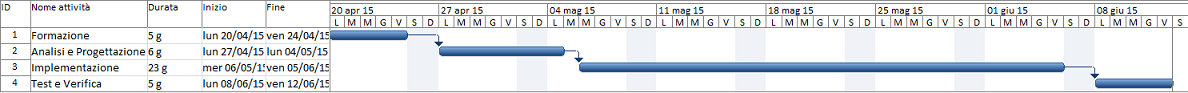
\includegraphics[width=1.1\columnwidth]{gantt_iniziale} 
    \caption{Diagramma Gantt della pianificazione iniziale}
\end{figure}

\subsection{Fase 1: Formazione (40 ore)}
Scopo: formazione sulle problematiche e tecnologie che si incontreranno durante lo stage.
In dettaglio:
\begin{itemize}
	\item angularjs, rest angular, jasmine, istanbul;
	\item ambiente di sviluppo IKS (\gls{ide} per Javascript PhpStorm, Git);
	\item linee guida per lo sviluppo e concetti di programmazione sicura;
	%\item principi di scrittura SOLID
	\item verifica competenze acquisite.
\end{itemize}
Output (oggetto di verifica per il passaggio alla fase successiva):
\begin{itemize}
	\item predisposizione ambiente di sviluppo;
	\item realizzazione di una web application di esempio che utilizzi le tecnologie e gli approcci
indicati.
\end{itemize}

\subsection{Fase 2: Analisi e Progettazione (40 ore)}
Scopo: analisi delle specifiche funzionali, definizione del piano di test e progettazione tecnica
della soluzione da realizzare.\\
In dettaglio:
\begin{itemize}
	\item analisi specifiche funzionali;
	\item progettazione di dettaglio;
	\item documentazione.
\end{itemize}
Output (oggetto di verifica per il passaggio alla fase successiva):
\begin{itemize}
	\item documento di Specifica Tecnica;
	\item User Stories.
\end{itemize}

\subsection{Fase 3: Implementazione (180 ore)}
Scopo: preparazione dell’ambiente di sviluppo e implementazione della soluzione.\\
In dettaglio:
\begin{itemize}
	\item implementazione tecnologica dei requisiti definiti in fase di analisi;
	\item documentazione.
\end{itemize}
Milestone settimanali:
\begin{enumerate}
	\item realizzazione delle funzionalità di dialogo REST con il backend;
	\item creazione dell'interfaccia del profilo utente singolo;
	\item visione della gerarchia aziendale e dell'organizzazione per progetti dell'organico;
	\item gestione operazioni \gls{crud} sui vari progetti aziendali e sui membri partecipanti.
\end{enumerate}
Output (oggetto di verifica per il passaggio alla fase successiva):
\begin{itemize}
	\item prodotto finale completo in tutte le sue parti;
	\item sorgenti commentati e pubblicati nel repository dei sorgenti aziendale.
\end{itemize}

\subsection{Fase 4: Test e Verifica (40 ore)}
Scopo: Verifica funzionale, dei requisiti e stesura della documentazione.\\
In dettaglio:
\begin{itemize}
	\item analisi dei risultati;
	\item verifica funzionale;
	\item verifica dei requisiti di progetto;
	\item revisione e correzione di eventuali bug;
	\item documentazione;
	\item verifica finale.
\end{itemize}
Output (oggetto di verifica per la conclusione del progetto):
\begin{itemize}
	\item documento finale (conclusioni sull'attività di Stage svolta, con obiettivi raggiunti e
conoscenze acquisite);
	\item eliminazione di bug riscontrati e pubblicazione delle modifiche nel repository dei sorgenti aziendale.
\end{itemize}